% XDSM of SizingLoopL1 -- one state variable, W_TO.
% Built from src/sizing/SizingLoopL1.m. Citation: Martins, design slide 6.
\documentclass[border=6pt, tikz]{standalone}
\usepackage[T1]{fontenc}
\usepackage{lmodern}
\usepackage{amsmath}
% xdsm_style.tex -- a small, self-contained XDSM style in TikZ.
%
% XDSM = eXtended Design Structure Matrix.
%   Lambe, A. B. and Martins, J. R. R. A., "Extensions to the Design Structure
%   Matrix for the Description of Multidisciplinary Design, Analysis, and
%   Optimization Processes", Structural and Multidisciplinary Optimization,
%   Vol. 46, 2012, pp. 273-284.
%
% Reading rule:
%   * Diagonal cells are COMPONENTS (something that computes).
%   * Off-diagonal cells are DATA. The cell in row i, column j carries data
%     produced by component i and consumed by component j.
%   * ABOVE the diagonal is feed-forward: data moves to a later component.
%   * BELOW the diagonal is FEEDBACK: data moves back to an earlier one.
%     Feedback is what makes the process a loop.
%   * The grey L-shaped highway is the data path: out of a component along its
%     row, then down or up its column into the consumer.
%   * The number in the corner of a component is its place in the process.
%
% There is no pyXDSM here on purpose: this file has no dependency beyond
% TikZ, so the diagrams rebuild with a plain TeX Live installation.

\usetikzlibrary{shapes.geometric, arrows.meta, positioning, matrix, backgrounds, fit, calc}

% ---- palette ------------------------------------------------------------
\definecolor{xdsmDriver}{RGB}{200, 221, 242}   % blue   -- the loop itself
\definecolor{xdsmAnalysis}{RGB}{212, 239, 213} % green  -- a discipline model
\definecolor{xdsmFunction}{RGB}{255, 231, 186} % orange -- an equation, no state
\definecolor{xdsmData}{RGB}{245, 245, 245}     % grey   -- data in transit
\definecolor{xdsmLine}{RGB}{140, 140, 140}
\definecolor{xdsmFeedback}{RGB}{192, 72, 40}

% ---- node styles --------------------------------------------------------
\tikzset{
  XBase/.style        = {draw, align=center, inner sep=3pt, font=\footnotesize,
                         minimum height=9mm, text width=26mm},
  Driver/.style       = {XBase, rectangle, rounded corners=6pt, very thick,
                         fill=xdsmDriver, double, double distance=1pt},
  Analysis/.style     = {XBase, rectangle, rounded corners=6pt, thick,
                         fill=xdsmAnalysis},
  Function/.style     = {XBase, rectangle, rounded corners=6pt, thick,
                         fill=xdsmFunction},
  Data/.style         = {draw, align=center, inner sep=2.5pt, font=\scriptsize,
                         trapezium, trapezium left angle=78, trapezium right angle=102,
                         trapezium stretches body, fill=xdsmData,
                         minimum height=7.5mm, text width=23mm},
  Output/.style       = {Data, fill=white, draw=black!55, dashed},
  DataLine/.style     = {line width=1.5pt, color=xdsmLine},
  FeedbackLine/.style = {line width=1.5pt, color=xdsmFeedback},
  StepNo/.style       = {font=\scriptsize\bfseries, inner sep=1pt,
                         fill=white, draw=black!40, rounded corners=1pt},
  XMatrix/.style      = {matrix of nodes, nodes in empty cells,
                         column sep=5mm, row sep=5mm,
                         nodes={anchor=center}},
}

% ---- helpers ------------------------------------------------------------
% \xdata{i}{j}   grey L-path: out of component i along row i to cell (i,j),
%                then along column j into component j.  Feed-forward.
\newcommand{\xdata}[2]{%
  \begin{scope}[on background layer]
    \draw[DataLine] (xdsm-#1-#1) -- (xdsm-#1-#2) -- (xdsm-#2-#2);
  \end{scope}}

% \xfeedback{i}{j}  the same path, drawn in the feedback colour.
\newcommand{\xfeedback}[2]{%
  \begin{scope}[on background layer]
    \draw[FeedbackLine] (xdsm-#1-#1) -- (xdsm-#1-#2) -- (xdsm-#2-#2);
  \end{scope}}

% \xstep{row}{col}{n}  put a process number on the block at (row,col).
\newcommand{\xstep}[3]{%
  \node[StepNo, anchor=south east] at ([xshift=1.5pt, yshift=-0.5pt]xdsm-#1-#2.north west) {#3};}

% ---- legend -------------------------------------------------------------
\newcommand{\xdsmlegend}{%
  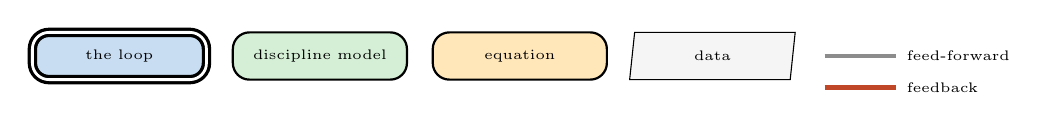
\begin{tikzpicture}[baseline]
    \node[Driver,   text width=20mm, minimum height=6mm, font=\tiny] (a) at (0,0)   {the loop};
    \node[Analysis, text width=20mm, minimum height=6mm, font=\tiny, right=3mm of a] (b) {discipline model};
    \node[Function, text width=20mm, minimum height=6mm, font=\tiny, right=3mm of b] (c) {equation};
    \node[Data,     text width=18mm, minimum height=6mm, font=\tiny, right=3mm of c] (d) {data};
    \draw[DataLine]     ([xshift=4mm]d.east) -- ++(9mm,0) node[right, font=\tiny, black] {feed-forward};
    \draw[FeedbackLine] ([xshift=4mm,yshift=-4mm]d.east) -- ++(9mm,0) node[right, font=\tiny, black] {feedback};
  \end{tikzpicture}}


\begin{document}
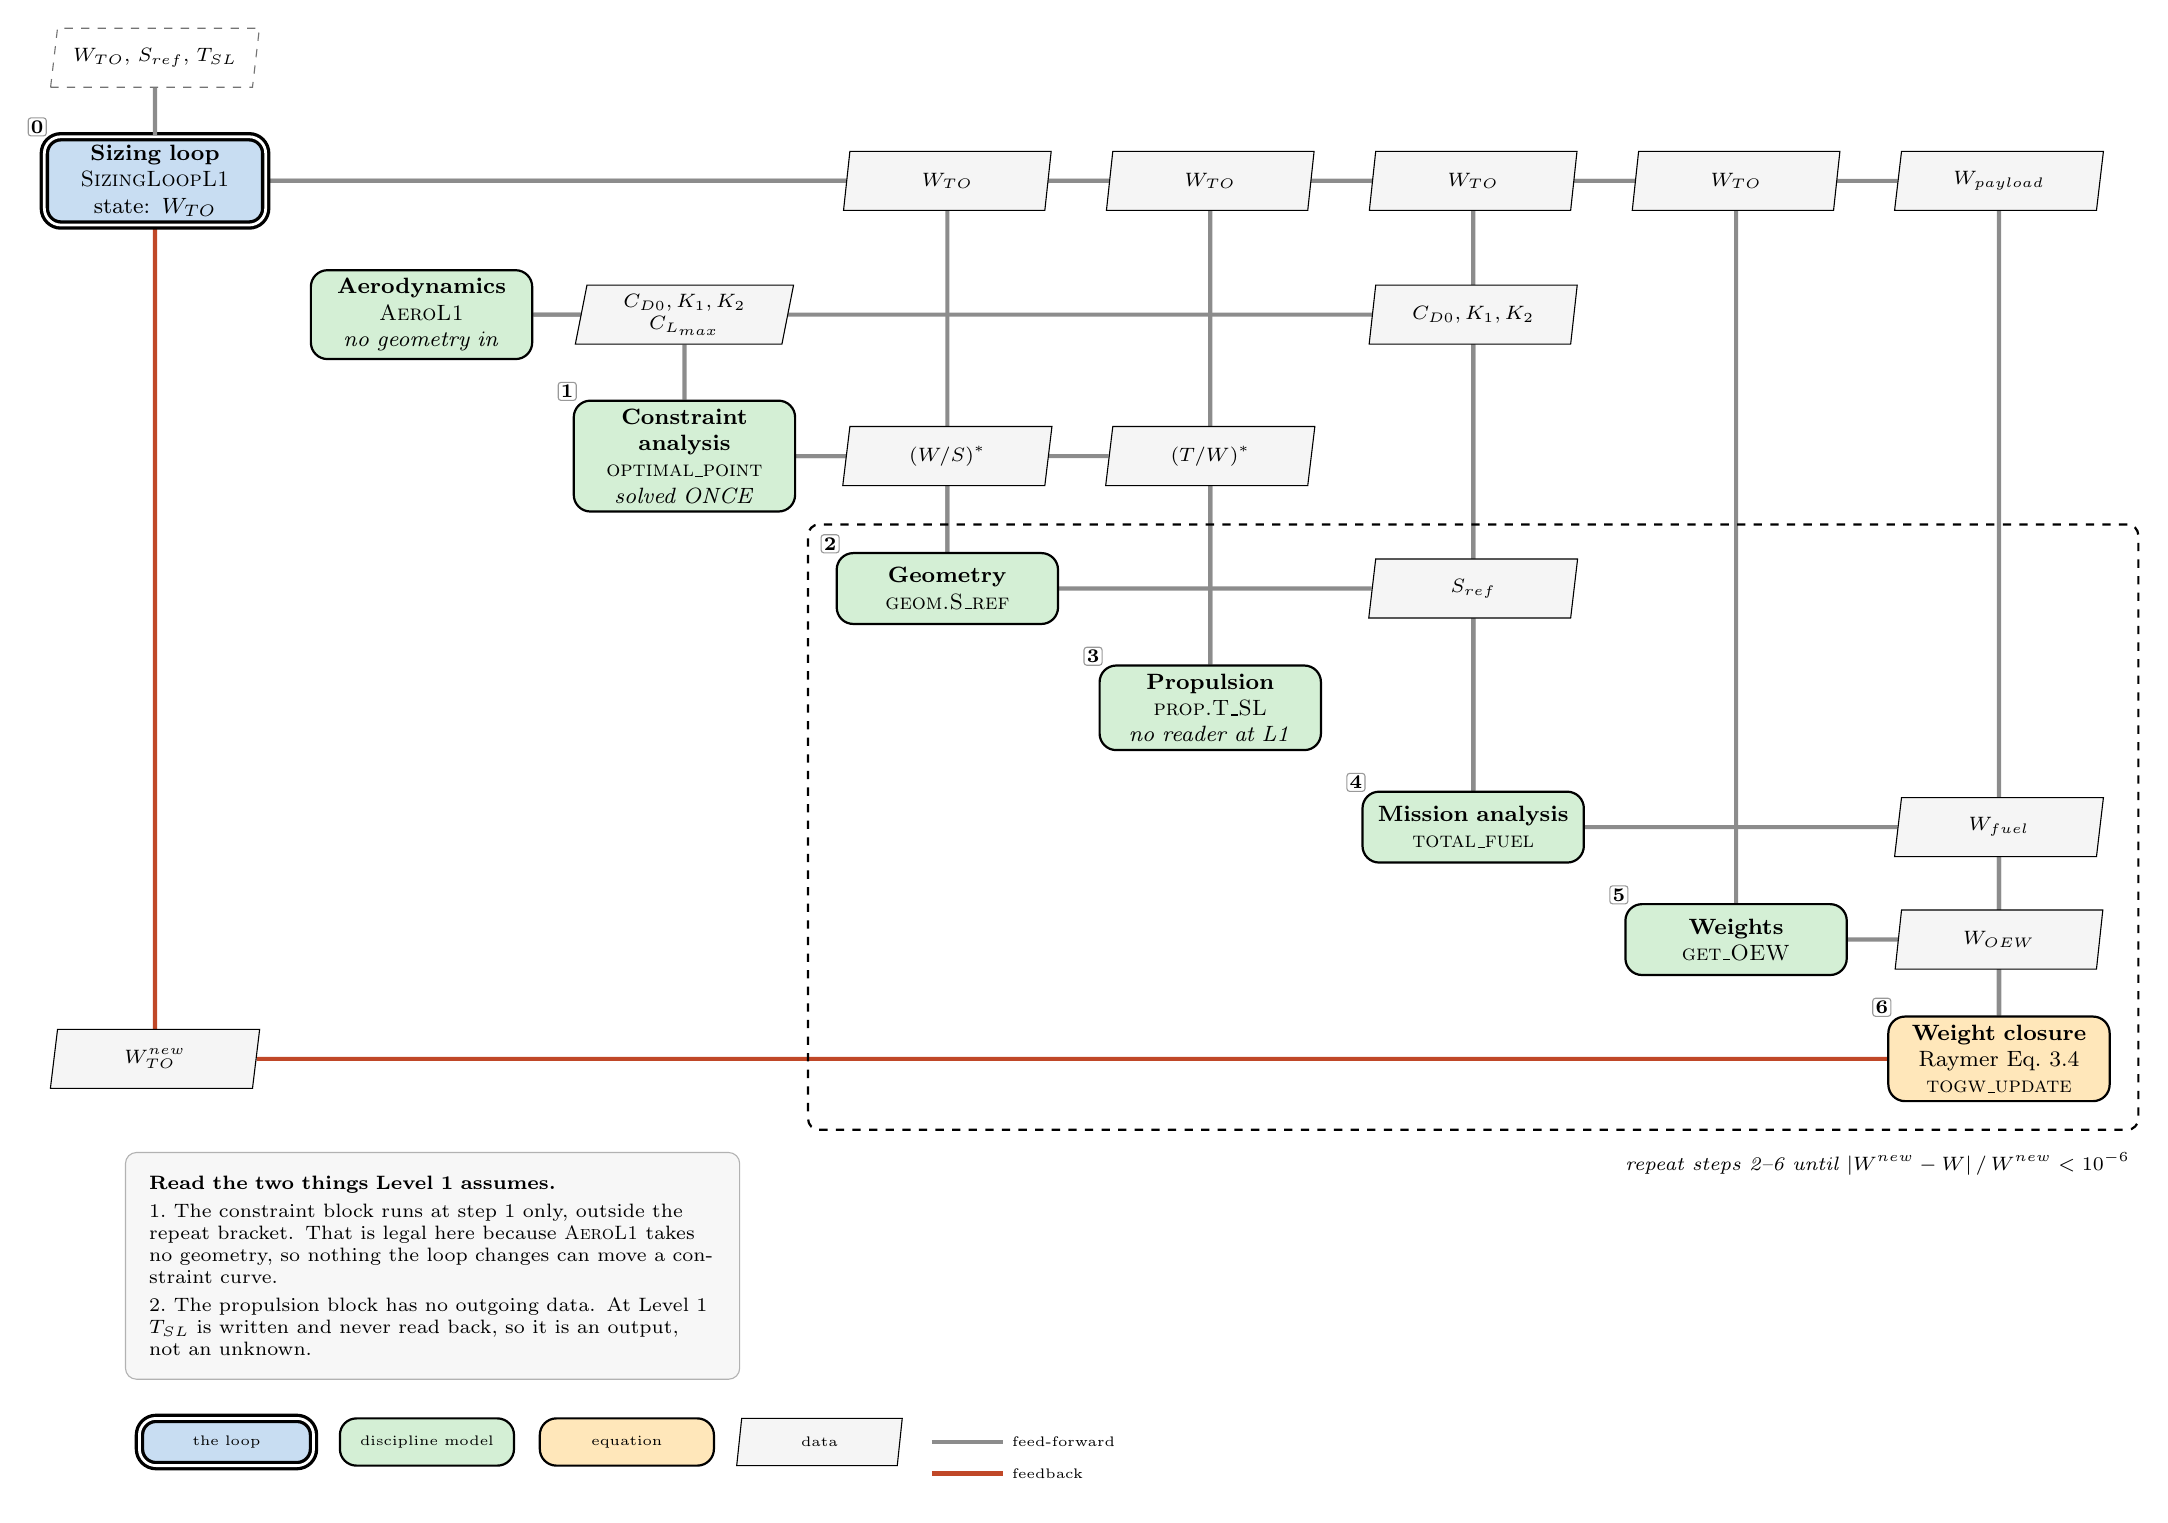
\begin{tikzpicture}

\matrix[XMatrix] (xdsm) {
% ------ 1 driver ---- 2 aero ------- 3 constraint -- 4 geom ------ 5 prop ------- 6 mission ---- 7 weights ---- 8 closure
  |[Driver]| {\textbf{Sizing loop}\\ \textsc{SizingLoopL1}\\ state: $W_{TO}$}
  & &
  & |[Data]| {$W_{TO}$}
  & |[Data]| {$W_{TO}$}
  & |[Data]| {$W_{TO}$}
  & |[Data]| {$W_{TO}$}
  & |[Data]| {$W_{payload}$} \\
%
  &
  |[Analysis]| {\textbf{Aerodynamics}\\ \textsc{AeroL1}\\ \emph{no geometry in}}
  & |[Data]| {$C_{D0},K_1,K_2$\\ $C_{L_{max}}$}
  & & &
  |[Data]| {$C_{D0},K_1,K_2$}
  & & \\
%
  & &
  |[Analysis]| {\textbf{Constraint analysis}\\ \textsc{optimal\_point}\\ \emph{solved ONCE}}
  & |[Data]| {$(W/S)^*$}
  & |[Data]| {$(T/W)^*$}
  & & & \\
%
  & & &
  |[Analysis]| {\textbf{Geometry}\\ \textsc{geom.S\_ref}}
  & &
  |[Data]| {$S_{ref}$}
  & & \\
%
  & & & &
  |[Analysis]| {\textbf{Propulsion}\\ \textsc{prop.T\_SL}\\ \emph{no reader at L1}}
  & & & \\
%
  & & & & &
  |[Analysis]| {\textbf{Mission analysis}\\ \textsc{total\_fuel}}
  & &
  |[Data]| {$W_{fuel}$} \\
%
  & & & & & &
  |[Analysis]| {\textbf{Weights}\\ \textsc{get\_OEW}}
  & |[Data]| {$W_{OEW}$} \\
%
  |[Data]| {$W_{TO}^{new}$}
  & & & & & & &
  |[Function]| {\textbf{Weight closure}\\ Raymer Eq.~3.4\\ \textsc{togw\_update}} \\
};

% ---- data highway: feed-forward ----------------------------------------
\xdata{1}{4}\xdata{1}{5}\xdata{1}{6}\xdata{1}{7}\xdata{1}{8}
\xdata{2}{3}\xdata{2}{6}
\xdata{3}{4}\xdata{3}{5}
\xdata{4}{6}
\xdata{6}{8}
\xdata{7}{8}

% ---- the one feedback edge: this is why it is a loop --------------------
\xfeedback{8}{1}

% ---- process order ------------------------------------------------------
\xstep{1}{1}{0}
\xstep{3}{3}{1}
\xstep{4}{4}{2}
\xstep{5}{5}{3}
\xstep{6}{6}{4}
\xstep{7}{7}{5}
\xstep{8}{8}{6}

% ---- the repeat bracket -------------------------------------------------
\node[draw, dashed, thick, rounded corners, inner sep=3.5mm,
      fit=(xdsm-4-4)(xdsm-8-8)(xdsm-4-6)(xdsm-7-8)] (rpt) {};
\node[font=\scriptsize\itshape, anchor=north east]
      at ([yshift=-1.5mm]rpt.south east)
      {repeat steps 2--6 until $|W^{new}-W| \,/\, W^{new} < 10^{-6}$};

% ---- outputs ------------------------------------------------------------
\node[Output, above=6mm of xdsm-1-1] (out) {$W_{TO}$, $S_{ref}$, $T_{SL}$};
\draw[DataLine] (xdsm-1-1) -- (out);

% ---- the teaching note --------------------------------------------------
\node[align=left, font=\scriptsize, anchor=north west, text width=72mm,
      draw=black!30, fill=black!3, rounded corners, inner sep=3mm]
  at ([yshift=-8mm]xdsm-8-1.south west)
  {\textbf{Read the two things Level 1 assumes.}\\[2pt]
   1.~The constraint block runs at step~1 only, outside the repeat bracket.
   That is legal here because \textsc{AeroL1} takes no geometry, so nothing
   the loop changes can move a constraint curve.\\[2pt]
   2.~The propulsion block has no outgoing data. At Level~1 $T_{SL}$ is
   written and never read back, so it is an output, not an unknown.};

\node[anchor=north west, font=\scriptsize] at ([yshift=-40mm]xdsm-8-1.south west) {\xdsmlegend};

\end{tikzpicture}
\end{document}
